% primary responsibility: Chaitu

\subsection{Reporting}

The second goal of this project is to provide parents with the ability to
monitor and derive reports on their child's Internet access.
%
We looked at incorporating BASE (Basic Analysis and Security Engine) into
Kindsicher to render this functionality.
%
BASE is based of the ACID (Analysis Console for Intrusion Databases) project
and provides a web-based front-end to query and analyze alerts generated by the
SNORT IDS system.

We first define a rule within SNORT to capture all HTTP traffic originating
from the home network.

\verb+alert tcp any any <> any 80 (msg:"HTTP Alert")+

This causes SNORT to log all HTTP requests from any source IP and port to any
destination IP and port 80 (indicating HTTP) to a MySQL database.
%
BASE then reads the alert information from this database and displays it in a
web-browser. Figure~\ref{fig:r1} shows this interaction.

\begin{figure}[!t]
    \centering
    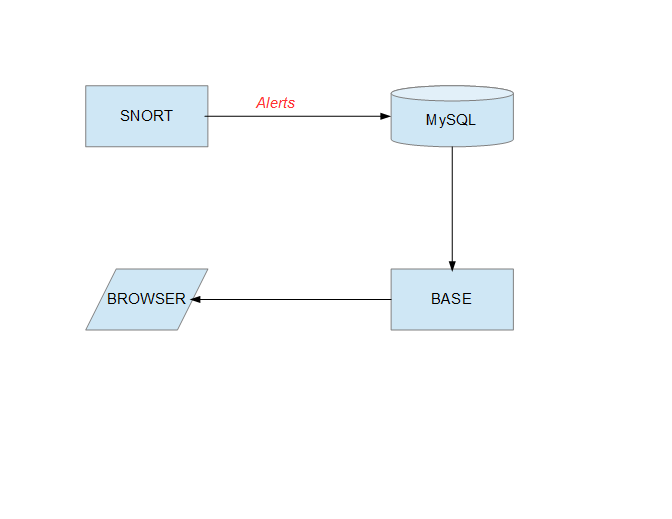
\includegraphics[width=\columnwidth]{figures/R1_BASE_Flow}
    \caption{The flow of data for BASE. Snort stores alerts into a database
    which BASE reads from. Base is accessed through a web browser.}
    \label{fig:r1}
\end{figure}

To access base you need to open a browser window and type in \texttt{<base server
name>/base} in the URL field.
%
Figure~\ref{fig:r2} shows the BASE home page presented to an user on logging
into BASE.

\begin{figure*}[!t]
    \centering
    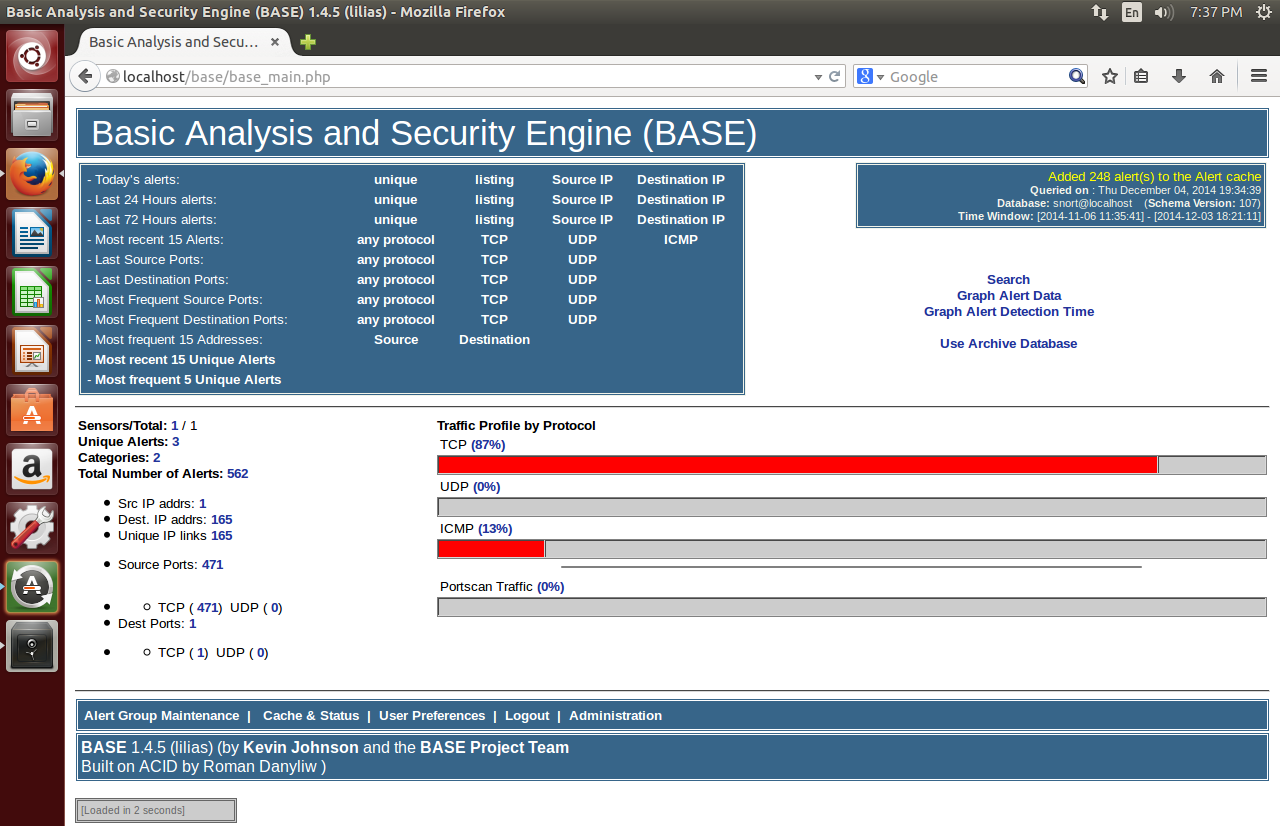
\includegraphics[width=1.7\columnwidth]{figures/R2_BASE_Main}
    \caption{A screenshot of the BASE home page.}
    \label{fig:r2}
\end{figure*}

For this project we were particularly interested in destination IP
addresses.
%
On clicking on the count of destination IP addresses shown in
Figure~\ref{fig:r2}, BASE displays a list of all the IP addresses accessed from
the home network (Figure~\ref{fig:r3}), along with other associated information
such as the number of times the IP was accessed and the number of source
addresses that accessed it.

\begin{figure*}[!tb]
    \centering
    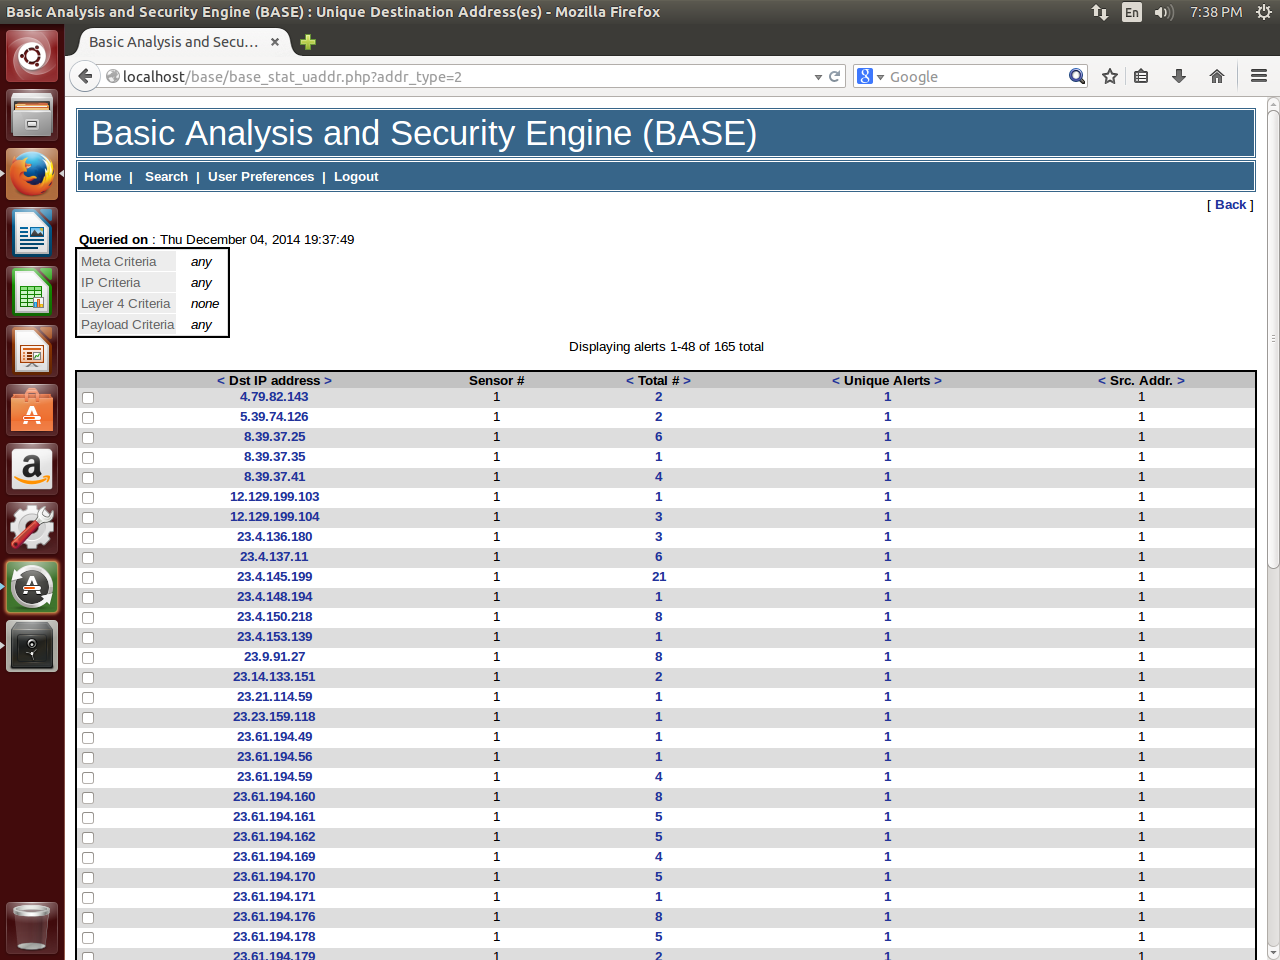
\includegraphics[width=1.7\columnwidth]{figures/R3_BASE_IPList}
    \caption{List of destination IPs accessed from the network as shown by
    BASE.}
    \label{fig:r3}
\end{figure*}

BASE also provides several canned reports to graphically represent
network data. Figure~\ref{fig:r4} shows an example of report selection and
parameter specification.

\begin{figure*}[!tb]
    \centering
    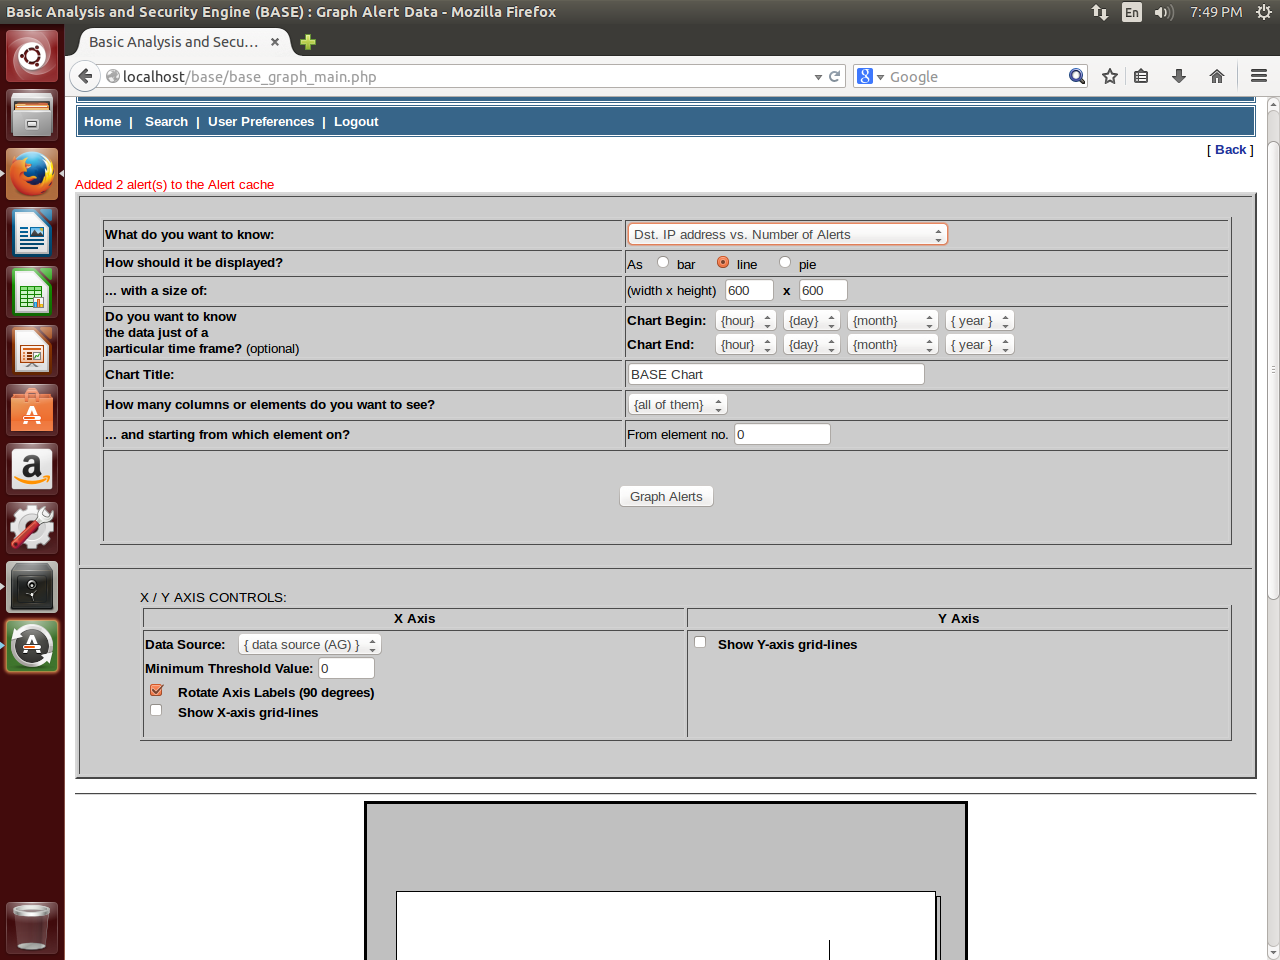
\includegraphics[width=1.7\columnwidth]{figures/R4_BASE_Report}
    \caption{BASE report selection and initiation.}
    \label{fig:r4}
\end{figure*}

Based on our study of BASE we came up with the following conclusions.

\textbf{Advantages of BASE:}
\begin{itemize}

\item It is built to work in conjunction with SNORT.

\item It provides a simple web-interface for users to view and
  analyze network traffic.

\item It comes with several in-built reports to help in the analysis.

\item Its open-source code is a useful starting point for customizations.

\end{itemize}

\textbf{Disadvantages of BASE:}
\begin{itemize}

\item It deals with only IP addresses and does not display the
  corresponding domain names.
  %
  IP addresses are not intuitive to users and this raises a real
  concern given the fact that our target users are parents who are not
  necessarily tech-savvy.

\item It also displays only the number of times a site has been
  accessed and gives no other information like the date and time of
  access.

\item The in-built reports do not support any correlation of which
  source IP(s) accessed which destination IP(s), reducing a parent's
  understanding of their child's Internet access.

\end{itemize}

Although BASE does provide an avenue for users to view and analyze web
access, it only partially meets the reporting goals for
Kindsicher because of these disadvantages.
%
This is further detailed in the Future Work/Improvements section.
%



